\section{Actividad No 06 – Funciones de Conversi\'on} 
		
\begin{enumerate}[1.]
	\item Crear un reporte que muestre lo siguiente por cada empleado.
	\\(Apellido del empleado) gana (Salario) pero quisiera (3 veces Salario).
	\\Etiquetar la columna como Sueldos Soñados.
	\\
	\\select 'Sueldos Soñados'=(last\_name + ' gana ' + Cast(salary as varchar(18)) + ' pero 
	\\quisiera ' + Cast((salary * 3) as varchar(18))) 
	\\from dbo.employees
	\\go
	\\
	\begin{center}
	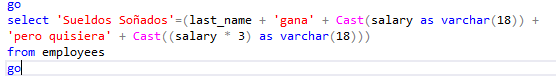
\includegraphics[width=5cm]{./Imagenes/actividad_06_01a}
	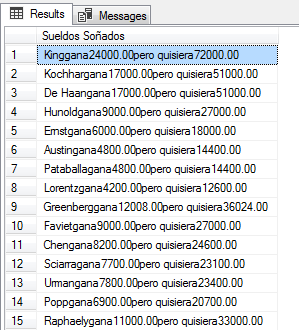
\includegraphics[width=5cm]{./Imagenes/actividad_06_01}
	\end{center}

	\item Realizar una consulta que muestre el Apellido del empleado, fecha de contratación y la Fecha de Revisión del Salario, la cual es el primer Lunes después de cada seis meses de servicio, etiquetar la columna como Revisión, asimismo el formato de esta fecha debe ser similar al siguiente: 
	\begin{center}
	Lunes, el veintiuno de julio, 2003 
	\end{center}
\
	\\select last\_name, hire\_date as Revision from employees 
	\\where hire\_date between '2003-06-17' and '2005-09-21';
	\\go
	
	\begin{center}
	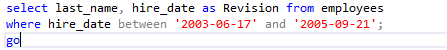
\includegraphics[width=5cm]{./Imagenes/actividad_06_02a}
	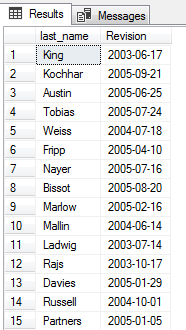
\includegraphics[width=5cm]{./Imagenes/actividad_06_02}
	\end{center}

	\item Mostrar un reporte que tenga los Apellidos, Fecha de Contrataci\'on y el D\'ia de Inicio de cada empleado (Lunes, Martes, etc…), etiquetar la \'ultima columna como D\'ia. Ordenar los resultados por el D\'ia de Inicio empezando por Lunes.
	\\
	\\select e.last\_name, e.hire\_date, DateName(WEEKDAY, jh.START\_DATE)as 'Dia' 
	\\from dbo.employees as e inner join dbo.job\_history as jh on 
	\\e.employee\_id=jh.employee\_id
	\\go
	\\
	\begin{center}
	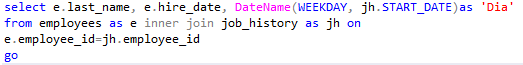
\includegraphics[width=5cm]{./Imagenes/actividad_06_03a}
	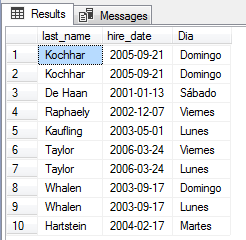
\includegraphics[width=5cm]{./Imagenes/actividad_06_03}
	\end{center}

\end{enumerate}

